
\documentclass[11pt]{beamer}
\usepackage{helvet} %font
\beamertemplatenavigationsymbolsempty
\usetheme{JuanLesPins}
\usefonttheme{structurebold}

\usepackage[french]{babel}
\usepackage[utf8]{inputenc}
\usepackage[T1]{fontenc}
\usepackage{amssymb,amsmath}
\usepackage{tikz}
\usepackage{geometry}
\usepackage{xcolor,colortbl}
\usetikzlibrary{arrows,positioning}
\usepackage{listings}

\AtBeginSubsection[]
{
   \begin{frame}
	\small \tableofcontents[currentsection]
   \end{frame}
}

\newenvironment{slide}[1]{%
\begin{frame}[environment=slide]
\frametitle{#1}
}{%
\end{frame}
}
\setbeamercolor{structure}{fg=red}
\setbeamercolor{frametitle}{bg=black,fg=white}
\definecolor{gris}{gray}{0.6}
\definecolor{grisclair}{gray}{0.9}

\newtheorem{exercice}{Exercice}

\title{Machine Learning V \\ Classification supervisée}
\author{Nicolas Bourgeois}
\date{}

\newcommand{\Python}[1]{
	{\small	\lstinputlisting[language=Python]{./#1.py}}
}
\newenvironment{pyenvsmall}
	{ \ttfamily \tiny }
	{\par  }

\newcommand{\Pythonsmall}[1]{
	{\scriptsize \lstinputlisting[language=Python]{./#1.py}}
}
\newcommand{\elimine}[1]{{\textcolor{lightgray}{#1}}}

\newcommand\Wider[2][3em]{%
\makebox[\linewidth][c]{%
  \begin{minipage}{\dimexpr\textwidth+#1\relax}
  \raggedright#2
  \end{minipage}%
  }%
}

\begin{document}

\begin{frame}
\maketitle
\end{frame}

\begin{frame}{SVM : objectif}

On dispose d'un ensemble d'observations ($\tilde{X},\tilde{Y}$).

\pause
\vspace{0.2cm}

On veut produire une partition de l'espace des X potentiels selon Y, par exemple avec des hyperplans.\\
\pause
\vspace{0.2cm}

Pour optimiser la robustesse on cherche à séparer au maximum les données d'entraînement.

$$\max_{\mathcal{H}}\sum _{x \in X} \min_{y \in \mathcal{H}} ||x-y||^2$$

\end{frame}

\begin{frame}{Exemple}
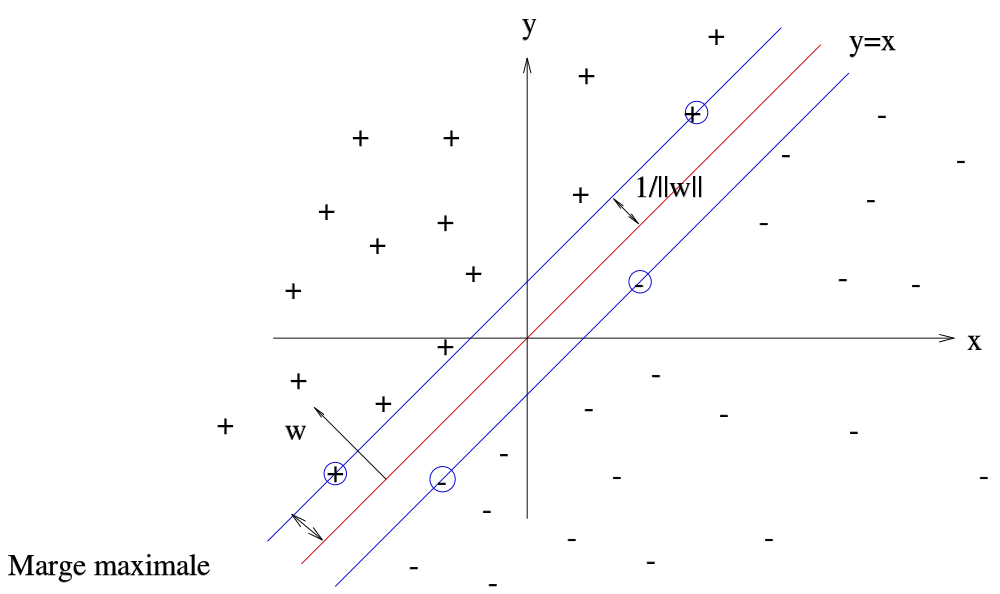
\includegraphics[scale=0.3]{svm}
\end{frame}


\begin{frame}{Exercice}
\begin{exercice}
Importez les données digits avec \texttt{dataset.load\_digits}. Divisez votre échantillon en deux parties. Effectuez un svm pour identifier les chiffre et testez sur l'échantillon de test.
\end{exercice}
\begin{exercice}
Comparez avec le résultat obtenu si on limite fortement le nombre d'itérations (10)
\end{exercice}
\end{frame}

\begin{frame}{Résultat attendu}
1.0 0.3212045169385194 \\
1 3 0 5 3 6 3 6 1 3 3 4 3 7 3 3 2 3 5 3 3 3 3 3 3 3 3 9 8 0 \\
1 4 0 5 3 6 9 6 1 7 5 4 4 7 2 8 2 2 5 7 9 5 4 4 9 0 8 9 8 0 \\
\vspace{0.2cm}
0.998 0.8983688833124216 \\
1 4 0 5 3 6 5 6 1 7 5 4 4 7 2 8 2 2 5 7 9 5 5 4 9 0 8 9 8 0 \\
1 4 0 5 3 6 9 6 1 7 5 4 4 7 2 8 2 2 5 7 9 5 4 4 9 0 8 9 8 0

\end{frame}

\begin{frame}{Solution}
\Pythonsmall{ex500}
\end{frame}

\begin{frame}{Exercice}
\begin{exercice}
Importez les données iris avec \texttt{dataset.load\_iris}. Divisez votre échantillon en deux parties. Effectuez un svm linéaire pour séparer les trois types de fleurs et testez le.
\end{exercice}
\begin{exercice}
Représentez côte à côte les valeurs observées $(\tilde{X},\tilde{Y})$ et le résultat de la prédiction (dans ce dernier on utilisera l'opacité pour distinguer les échantillons d'apprentissage et de test) 
\end{exercice}
\end{frame}

\begin{frame}{Résultat attendu}
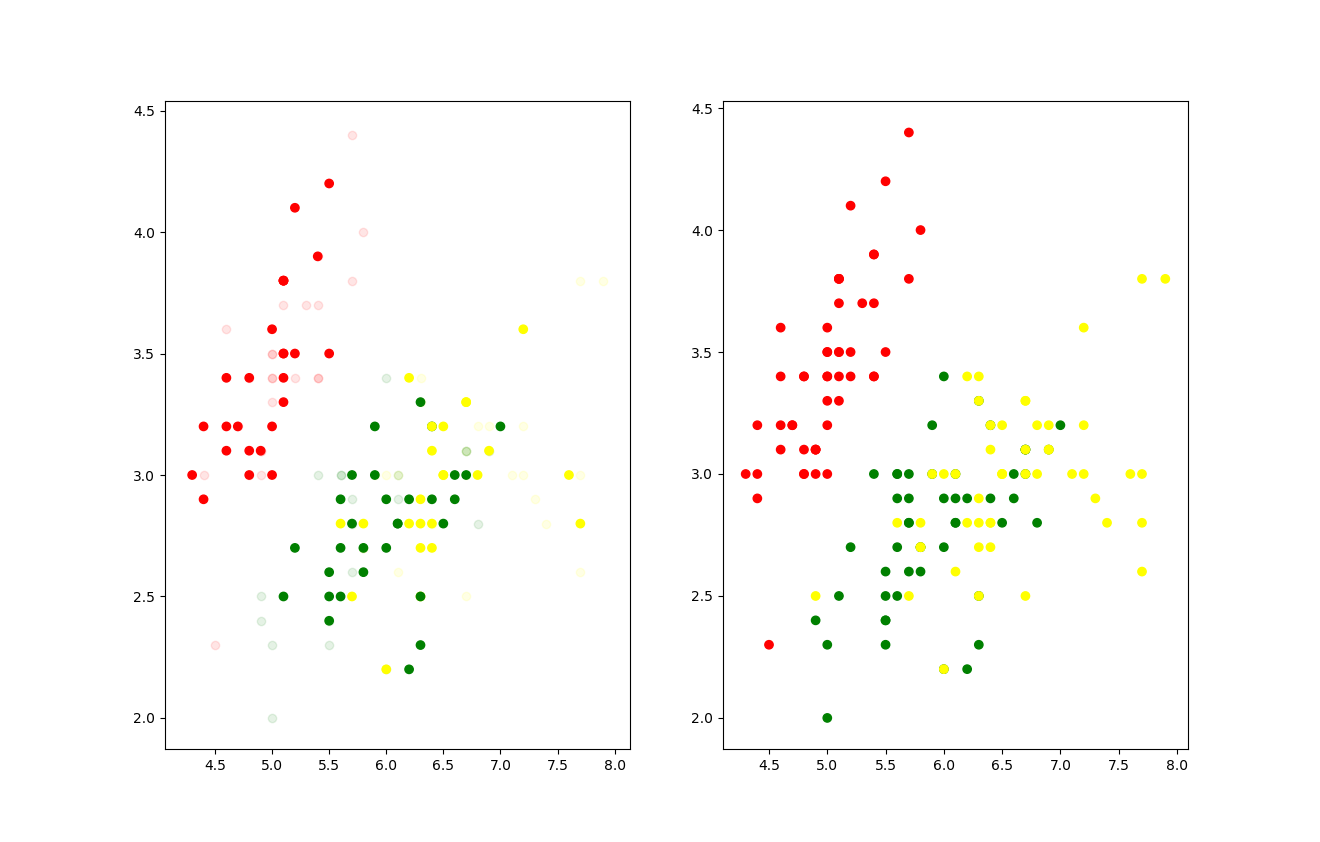
\includegraphics[scale=0.35]{ex502}
\end{frame}

\begin{frame}{Solution}
\vspace{-0.3cm}
\Pythonsmall{ex502}
\end{frame}

\begin{frame}{Exercice}
\begin{exercice}
Effectuez la même manipulation avec les données \textit{age} et \textit{fare} du titanic, en vérifiant si vous prédisez bien \textit{survived}.
\end{exercice}

\begin{exercice}
Même chose, mais en intégrant la variable \textit{sex} (numérisée) dans l'apprentissage.
\end{exercice}
\end{frame}

\begin{frame}{Résultat attendu (1)}
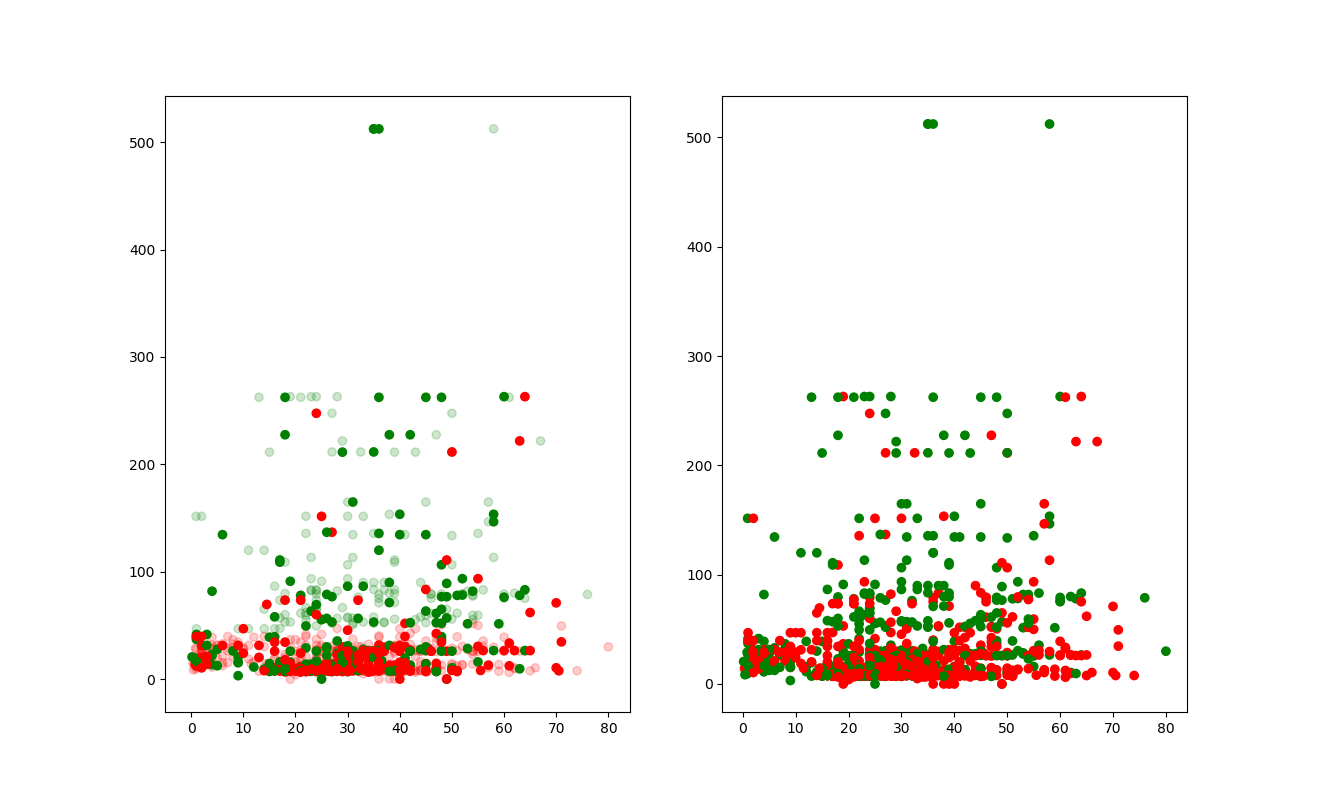
\includegraphics[scale=0.35]{ex507}
\end{frame}

\begin{frame}{Résultat attendu (2)}
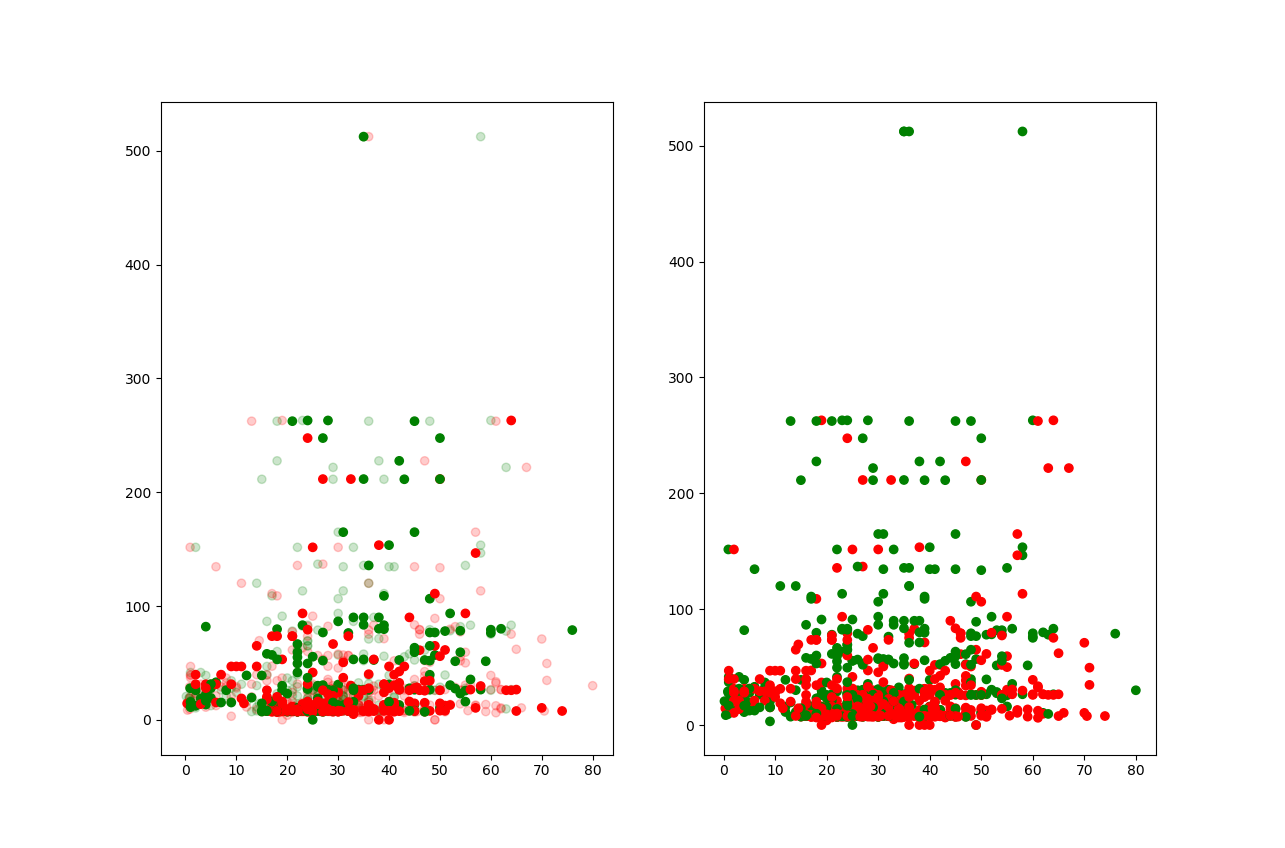
\includegraphics[scale=0.35]{ex508}
\end{frame}

\begin{frame}{Solution (1)}
\vspace{-0.3cm}
\Pythonsmall{ex507}
\end{frame}

\begin{frame}{Solution (2)}
\vspace{-0.3cm}
\Pythonsmall{ex508}
\end{frame}


\begin{frame}{Régression logistique : objectif}

On dispose d'un ensemble d'observations ($\tilde{X},\tilde{Y}$) où $\tilde{X}$ est numérique et $\tilde{Y}$ binaire.

\pause
\vspace{0.2cm}

On veut produire une fonction explicite Y=f(X).\\
\pause
\vspace{0.2cm}

Dont le logit est linéaire:

$$\ln {\frac {p(Y=1\vert X)}{p(Y=0\vert X)}}=a_{0}+a_{1}X_{1}+...+a_{k}X_{k}$$
\end{frame}


\begin{frame}{Exercice}
\begin{exercice}
Importez les données du titanic. Entraînez une régression logistique sur la variable de survie à partir de l'age, du prix du billet et du genre.
\end{exercice}
\end{frame}

\begin{frame}{Résultat attendu}
0.7875 0.7782945736434108\\
\vspace{0.2cm}
1 0 0 1 0 0 1 1 0 1 1 0 1 1 0 1 1 1 0 1 0 0 1 1 1 1 0 0 0 1\\
1 1 1 1 0 0 1 1 1 1 1 1 1 1 1 1 1 1 0 1 0 0 1 1 1 1 0 1 1 1

\end{frame}

\begin{frame}{Solution}
\Pythonsmall{ex510}
\end{frame}


\end{document}